\section{Inteligencia Artificial}
\begin{frame}[plain] % plain para um slide sem cabeçalho ou rodapé
	\centering
	\vfill
	\textbf{\Huge Aprendizado Estatístico}
	\vfill
\end{frame}

\begin{frame}{O que é Inteligência Artificial (IA)?}
    \begin{block}{}
        \begin{itemize}
            \item Não há uma única forma de definir; 
            \item Diferentes autores a descrevem de maneiras distintas a depender do contexto em que está sendo empregada.
        \end{itemize}
    \end{block}
\end{frame}
% John Haugeland
\begin{frame}{O que é IA?}
    \begin{minipage}{0.5\linewidth}
        \begin{figure}
            \centering
            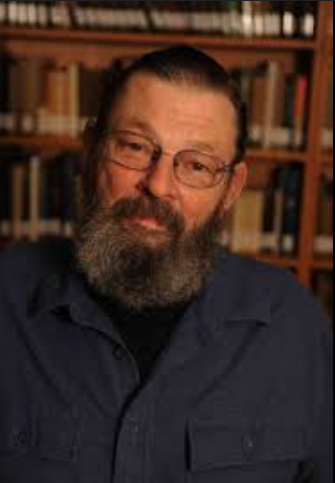
\includegraphics[width=0.6\linewidth]{imagens//secao1/haugeland1985.png}
            \caption{Prof. John Haugeland}
        \end{figure}
    \end{minipage}
    \begin{minipage}{0.5\linewidth}
        \begin{itemize}
        \justifying
            \item \textit{Artificial Intelligence: The Very Idea (1985).}
            \item \aspas{O novo e interessante esforço para fazer os
        computadores pensarem (...) máquinas com mentes, no
        sentido total e literal.}
        \end{itemize}
    \end{minipage}
\end{frame}

% Richard Bellman
\begin{frame}{O que é IA?}
    \begin{minipage}{0.5\linewidth}
        \begin{itemize}
        \justifying
            \item \textit{Artificial Intelligence (1972).}
            \item 
            \aspas{[Automatização de] atividades que associamos ao pensamento humano, atividades como a tomada de decisões, a resolução de problemas, o aprendizado...}
        \end{itemize}
    \end{minipage}
    \begin{minipage}{0.5\linewidth}
        \begin{figure}
            \centering
            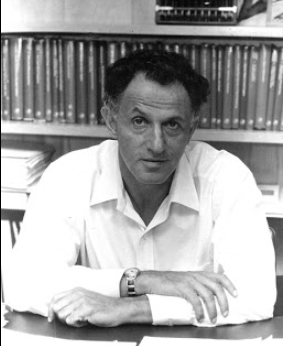
\includegraphics[width=0.6\linewidth]{imagens//secao1/bellman1978.png}
            \caption{Richard Bellman}
            \label{fig:enter-label}
        \end{figure}
    \end{minipage}
\end{frame}

% Raymond Kurzweil
\begin{frame}{O que é IA?}
    \begin{minipage}{0.5\linewidth}
        \begin{figure}
            \centering
            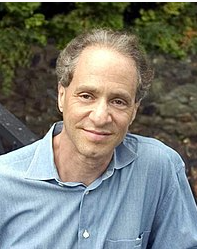
\includegraphics[width=0.5\linewidth]{imagens//secao1/kurzweil.png}
            \caption{Raymond Kurzweil}
        \end{figure}
    \end{minipage}
    \begin{minipage}{0.5\linewidth}
        \begin{itemize}
        \justifying
            \item \textit{The Age of Intelligent Machines (1990).}
            \item 
            \aspas{A arte de criar máquinas que executam funções que exigem inteligência quando executadas por pessoas.”}
        \end{itemize}
    \end{minipage}
\end{frame}

\begin{frame}{O que é IA? }
    \begin{itemize}
        \item
        \justifying 
        \aspas{
        O estudo das faculdades mentais pelo uso de modelos computacionais.
        }
        (Charniak e McDermott, 1985) 
        
        \item 
        \aspas{
        O estudo das computações que tornam possível perceber, raciocinar e agir.
        }
        (Winston, 1992)
        
        \item 
        \aspas{
        O estudo de como os computadores podem fazer tarefas que hoje são melhor desempenhadas pelas pessoas.
        }
        (Rich and Knight, 1991)
        
        \item 
        \aspas{
        “Inteligência Computacional é o estudo do projeto de agentes inteligentes.
        }
        (Poole et al., 1998) 
    \end{itemize}
\end{frame}

\begin{frame}{O que é IA?}
	\begin{block}{Segundo a Data Science Academy (DSA)}
		\justifying
		\aspas{Inteligência Artificial (IA) refere-se ao campo da ciência da computação que se concentra na criação de sistemas capazes de realizar tarefas que normalmente exigiriam inteligência humana.}
	\end{block}
\end{frame}

\begin{frame}{Inteligência Artificial VS Aprendizado Estatístico}
	\begin{block}{Definição}
		\justifying
		\aspas{Aprendizado de Máquina [ou Estatístico] é o campo de estudo da ciência da computação que dá ao computador a habilidade de \underline{aprender} sem ser explicitamente programado.}
		Arthur Samuel (1959)
	\end{block}
	\begin{block}{O que é aprender?}
		Se baixássemos todo o conteúdo da Wikipédia em um computador, poderíamos afirmar que ele aprendeu?
	\end{block}
\end{frame}

\begin{frame}{Inteligência Artificial VS Aprendizado Estatístico}
	\begin{block}{Exemplo}
		\justifying
		Suponha que desejamos criar um filtro de \textit{spam}.
		Uma forma de fazer isso seria seguindos os passos:
		\begin{enumerate}
			\justifying
			\item Examinar emails que sejam \textit{spam}.
			É provável que repitam-se as frases: \textit{para você, gratuito, oportunidade, imperdível...}
			\item Escrever um programa que busque por uma das palavras citadas acima no corpo do email e acione uma \textit{flag}.
			\item Testamos o programa e repetimos os passos 1 e 2 até nosso programa estar bom o suficiente. 
		\end{enumerate}
	\end{block}
\end{frame}

\begin{frame}{Inteligência Artificial VS Aprendizado Estatístico}
	\begin{figure}[h]
		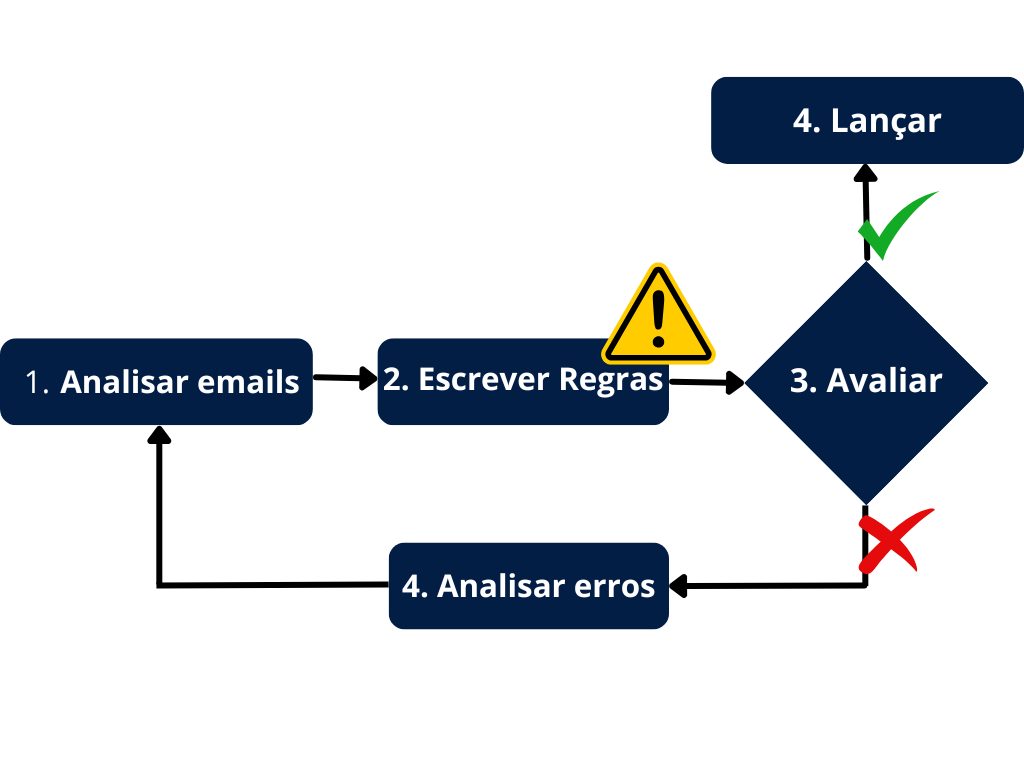
\includegraphics[scale=0.4]{imagens//secao1/tradicionalspam.png}
	\end{figure}
\end{frame}


\begin{frame}{Inteligência Artificial VS Aprendizado Estatístico}
	\begin{block}{Observações}
		\begin{itemize}
			\item Essa solução funciona? \textbf{SIM!!} \emoji{smile}; 
			\item É a melhor forma de fazer? \textbf{NÃO!!} \emoji{expressionless};
			\item Sensível a pequenas mudanças, e.g, Pra Você, PARA VOCÊ, PRA VOCE...
		\end{itemize}
	\end{block}
\end{frame}

\begin{frame}{Inteligência Artificial VS Aprendizado Estatístico}
	\begin{block}{Exemplo \textit{(Filtro de Spam)}}
		\justifying
		Outra abordagem seria:
		\begin{enumerate}
			\justifying
			\item Examinar emails que sejam \textit{spam};
			\item Treinar um modelo de aprendizado de máquina para classificar emails como \textit{spam} ou \textit{ham}.
		\end{enumerate}
	\end{block}
\end{frame}

\begin{frame}{Inteligência Artificial VS Aprendizado Estatístico}
	\begin{figure}[h]
		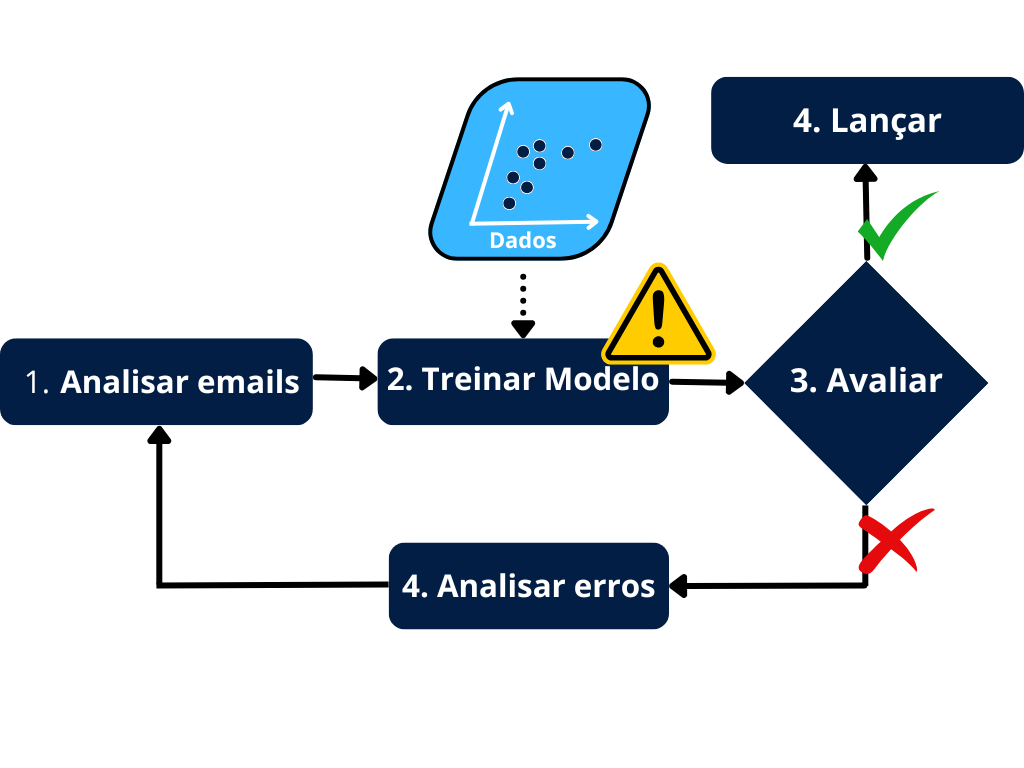
\includegraphics[scale=0.4]{imagens//secao1/mlspam.png}
	\end{figure}
\end{frame}

\begin{frame}{Inteligência Artificial VS Aprendizado Estatístico}
	\begin{figure}[h]
		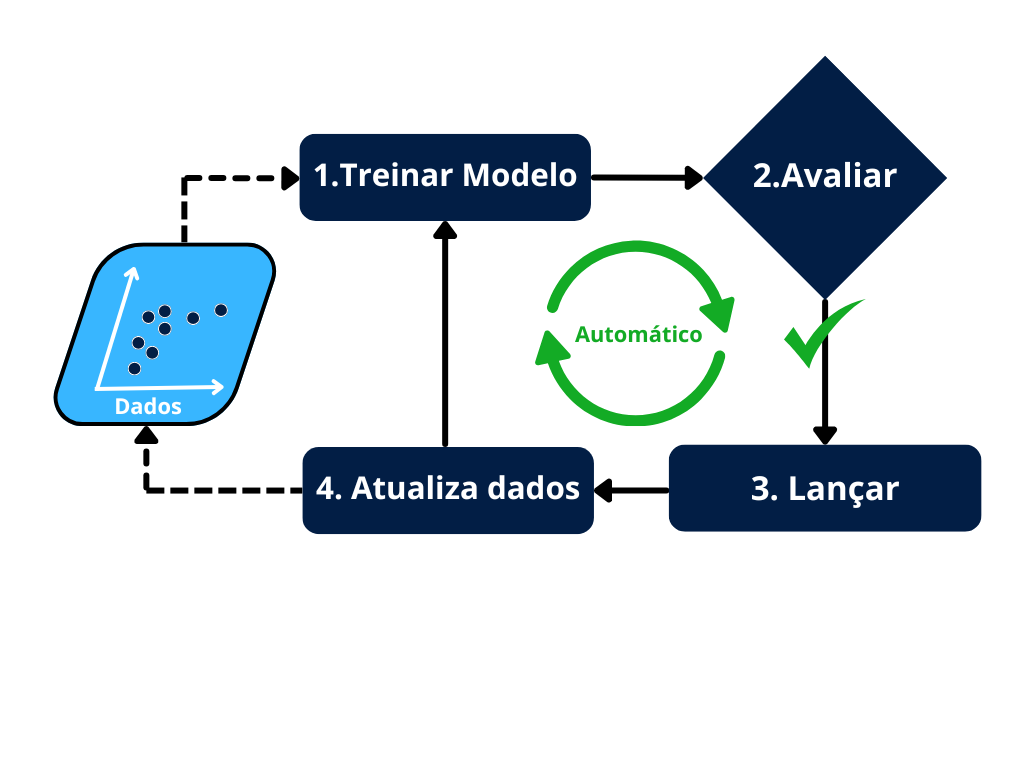
\includegraphics[scale=0.4]{imagens//secao1/automl.png}
	\end{figure}
\end{frame}
































